% 二体碰撞

\pentry{二体系统\upref{TwoBD}}

注意以下讨论的碰撞不必要求在一瞬间发生, 可以拓展到有限距离的作用力甚至无穷远但不断衰减的作用力. 例如考虑两个带电荷的质点的碰撞. 在无穷远处时, 二者之间的作用可忽略, 此时的速度可定义为初速度. 当发生相互作用后, 把两质点互相远离到相距无穷远时的速度定义为末速度.

\subsection{一维情况}
高中物理中, 若两质点的运动限制在同一直线上且碰撞为完全弹性碰撞, 我们可以联立能量守恒和动量守恒两条式子来解出碰撞后的速度. 但这里介绍另一种更简单的方法, 即利用质心系求解. 为了区别于质心系, 我们把原参考系叫做\bb{实验室参考系}(简称为实验系). 令两质点质量分别为 $m_1$ 和 $m_2$, 实验系中初速度分别为 $v_{10}$ 和 $v_{20}$, 需要求实验系中的末速度 $v_1$ 和 $v_2$. 根据定义, 系统质心的位置为 $x_c = (m_1 x_1 + m_2 x_2)/(m_1 + m_2)$, 等式两边对时间 $t$ 求导, 得质心的速度为
\begin{equation}\label{TwoCld_eq1}
v_c = (m_1 v_1 + m_2 v_2)/(m_1 + m_2)
\end{equation}
现在我们在质心系中考虑该问题. 在三维情况下, 质心系中的二体系统只有三个自由度(二体系统\upref{TwoBD}\autoref{TwoBD_eq3}), 不难类推在一维情况下二体系统只有一个自由度. 所以无论维度多少, 在质心系中考虑二体碰撞问题将会简单得多. 

由速度叠加原理%引用未完成
, 初始时两质点在质心系中的速度分别为
\begin{equation}
v_{c10} = v_{10} - v_c \qquad v_{c20} = v_{20} - v_c
\end{equation}
先考虑质心系中的完全弹性碰撞, 由于两质点的速度大小始终成正比 (质心系\upref{CM}\autoref{CM_eq8}), 为了使能量守恒, 碰撞只能有一种结果, 即两质点的速度方向都取反方向而速度大小保持不变. 现在我们重新回到实验系中, 两质点的末速度分别为
\begin{equation}
v_1 = v_c + (-v_{c10}) = 2v_c - v_{10}  \qquad v_2 = v_c + (-v_{c20}) = 2v_c - v_{20}
\end{equation}
代入\autoref{TwoCld_eq1} 即可得到最后结果.

若问题为非完全弹性碰撞, 可设质心系中碰撞后与碰撞前的能量比值为 $\alpha^2 < 1$, 即速度的比值为 $\alpha$. 碰撞后两质点的质心系速度分别变为 $-\alpha v_{c10}$ 和 $-\alpha v_{c20}$, 变换到实验系中速度为
\begin{equation}\ali{
v_1 = v_c + (-\alpha v_{c10}) = (1 + \alpha) v_c - \alpha v_{10}\\
v_2 = v_c + (-\alpha v_{c20}) = (1 + \alpha) v_c - \alpha v_{20}
}\end{equation}

\subsection{三维的情况}

\begin{figure}[ht]
\centering
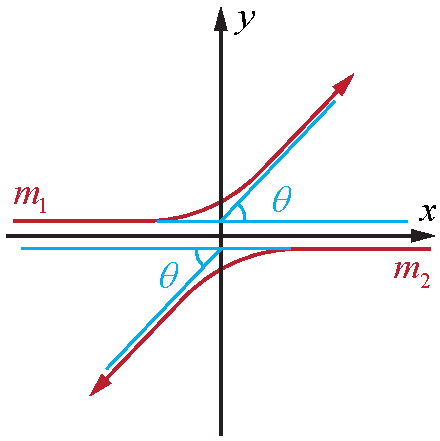
\includegraphics[width=5.5cm]{./figures/TwoCld.pdf}
\caption{质心系中的二体碰撞} \label{TwoCld_fig1}
\end{figure}

由于在多维情况下, 碰撞损失的能量可能与碰撞的角度有关, 这里仅讨论最常见的完全弹性碰撞.
碰撞的轨迹如\autoref{TwoCld_fig1}所示. 由于质心系中系统的总动量始终为 0( 质心系\upref{CM}\autoref{CM_eq8}),  初状态和末状态中两质点的速度方向相反, 但延长线一般不重合(否则就变为上面的一维情况). 质点末状态速度与初状态速度的夹角叫做\bb{散射角(scattering angle)}. 注意质心系中两质点散射角相同, 而实验系中两散射角不必相同. 求散射角需要知道具体的作用力形式, 以下讨论假设我们已知质心系中的散射角.%未完成 在理论力学中加上求散射角的方法, 参考 goldstein.
若两质点间的相互作用力与两点的连线共线, 那么质心系中两质点的运动轨迹将始终在同一平面上, 而这在实验系中一般不成立(当两个质点的入射延长线为两条不平行且不相交的直线时).

令质量分别为 $m_1$ 和 $m_2$ 的两质点初始速度为 $\vec v_{10}$ 和 $\vec v_{20}$, 为了方便, 我们规定质心系的 $x$ 轴与第一个质点在质心系中的入射方向相同, 则质心系中的初始速度分别为
\begin{equation}
\vec v_{c10} = (v_{10} - v_c)\uvec x \qquad \vec v_{c20} = (-v_{20} - v_c) \uvec x
\end{equation}
其中质心速度为
\begin{equation}
\vec v_c = (m_1 v_1 + m_2 v_2)\uvec x/(m_1 + m_2)
\end{equation}
完全弹性碰撞说明能量守恒, 类比一维的情况可得质心系中两质点末速度的大小分别等于初速度大小. 所以末速度分别为
\begin{equation}
\vec v_{c1} = (v_{10} - v_c)(\uvec x\cos\theta + \uvec y\sin\theta) \qquad
\vec v_{c2} = -(v_{20} + v_c)(\uvec x\cos\theta + \uvec y\sin\theta)
\end{equation}
最后再变换到实验系, 得末速度分别为
\begin{equation}
\vec v_1 = \vec v_c + \vec v_{c1} \qquad
\vec v_2 = \vec v_c + \vec v_{c2}
\end{equation}





